\documentclass[12pt]{article}
\usepackage{amssymb}
\usepackage[UTF8]{ctex}
\usepackage{geometry}
\usepackage{units}
\usepackage{pifont}
\geometry{
	a4paper,
	total={150mm,237mm},
	left=30mm,
	top=27mm,
	}
\usepackage{amsmath}
\usepackage{enumerate}
\usepackage{lipsum}
\usepackage{graphicx}
\usepackage{hyperref}
\usepackage{indentfirst}
\usepackage[graphicx]{realboxes}
\usepackage{booktabs}
\usepackage{cases}
\usepackage{subfig}  
\usepackage{float}
\lstset{language=C,
    basicstyle=\tt,
    %行号
    numbers=left,
    rulesepcolor=\color{red!20!green!20!blue!20},
    escapeinside=' ',
    xleftmargin=2em,xrightmargin=2em, aboveskip=1em,
    %背景框
    framexleftmargin=1.5mm,
    frame=shadowbox,
    %背景色
    backgroundcolor=\color[RGB]{255,255,255},
    %样式
    keywordstyle=\color{blue}\bfseries,
    identifierstyle=\bf,
    numberstyle=\color[RGB]{0,192,192},
    commentstyle=\it\color[RGB]{96,96,96},`'
    stringstyle=\rmfamily\slshape\color[RGB]{128,0,0},
    %显示空格
    showstringspaces=false
    }

\setlength{\parindent}{2em}
\title{Lab1}
\author{姓名:陈锐林,学号:21307130148}
\date{\today}
 
\begin{document}
\maketitle
\begin{Large}
    \noindent 一、代码:
\end{Large}
\begin{lstlisting}
    // pingpong.c
    #include "kernel/types.h"
    #include "kernel/stat.h"
    #include "user/user.h"
    int main() {
        int pp[2];  //管道
        int pid;     
    
        if (pipe(pp) == -1) {
            printf("pipe error"); //if pipe失败
            exit(1);
        }
        pid = fork(); // 创建子进程
        if (pid == -1) {
            printf("fork error"); //if fork失败
            exit(1);
        }
        if (pid == 0) { //子进程
            char buf;
            // 子进程等待接收数据
            read(pp[0], &buf, 1);
            printf("%d: received ping\n", getpid());
            // 子进程写回给父进程
            write(pp[1], &buf, 1);
            // 子进程退出
            exit(0);
        } else { // 父进程
            char buf = '!'; // 父进程要发送的数据
            // 父进程向管道中写入数据,传递给子进程
            write(pp[1], &buf, 1);
            // 父进程等待从子进程接收数据
            read(pp[0], &buf, 1);
            printf("%d: received pong\n", getpid());
            // 父进程退出
            exit(0);
        }
        return 0;
    }
\end{lstlisting}
\vspace*{1cm}
\begin{Large}
    \noindent 二、实验思路:\\
\end{Large}
\hspace*{2em}这个实验比较简单,思路也很清晰。根据题目要求,我们要利用一个管道在父进程和子进程之间传递数据(示意图如下)。大致步骤如下:pipe函数进行管道创建,根据fork返回的pid执行不同操作;父进程向管道中写入数据传递给子进程;子进程接收数据,并且发送回父进程。\\

\begin{figure}[htbp]
    \centering
    \includegraphics*[height=6cm,width=8cm]{HW1-1.jpg}\\
\end{figure}
\vspace*{1cm}
\begin{Large}
    \noindent 三、测试结果:
\end{Large}
\begin{figure}[htbp]
    \centering
    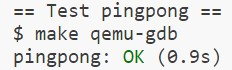
\includegraphics[height=2cm,width=6cm]{HW1.jpg}
\end{figure}\\
\noindent 经测试,0.9s可完成一次,即一秒钟内能完成大概1.11次该操作。
\end{document}